\documentclass{beamer}
\usepackage{amsmath,amssymb,amsthm,slashed, euscript, tikz, tikz-cd}



\textwidth=110mm


\title{Fundamental groups of $C^*$-algebras}
\institute
{
Noncommutative geometry and topology
}

\author{Petr R. Ivankov  }



\theoremstyle{plain}
\newtheorem{defn}{Definition}
\newtheorem{rem}{Remark}
\newtheorem{exm}{Example}
\newtheorem*{claim}{Claim}
\newtheorem{prop}{Proposition}
\newtheorem{empt}[prop]{}%[section]
\newtheorem{lem}{Lemma}%[section]
\newtheorem{thm}{Theorem}%[section]



\newcommand{\A}{\mathcal{A}}
\newcommand{\be}{\begin{equation}}
\newcommand{\ee}{\end{equation}}
\newcommand{\Ga}{\Gamma}
\newcommand{\B}{\mathcal{B}}
\newcommand{\Cc}{\mathcal{C}}
\newcommand{\C}{\mathbb{C}}
\newcommand{\D}{\mathcal{D}}
\newcommand{\G}{\mathcal{G}}
\newcommand{\Hc}{\mathcal{H}}
\newcommand{\Lc}{\mathcal{L}}
\newcommand{\Pc}{\mathcal{P}}
\newcommand{\Sc}{\mathcal{S}}
\newcommand{\U}{\mathcal{U}}
\newcommand{\rar}{\rightarrow}
\newcommand{\Ef}{\mathbb{E}}
\newcommand{\desc}{\mathfrak{desc}}


%Uppercase Gothic characters
\newcommand{\gtA}{\mathfrak{A}}
\newcommand{\gtB}{\mathfrak{B}}
\newcommand{\gtM}{\mathfrak{M}}
\newcommand{\gtN}{\mathfrak{N}}
\newcommand{\gtP}{\mathfrak{P}}
\newcommand{\gtS}{\mathfrak{S}}

%Lowercase Gothic characters
\newcommand{\gtf}{\mathfrak{f}}
\newcommand{\gtg}{\mathfrak{g}}

%Bold Characters
\newcommand{\Cb}{\mathbb{C}}
\newcommand{\Nb}{\mathbb{N}}
\newcommand{\Rb}{\mathbb{R}}
\newcommand{\Zb}{\mathbb{Z}}

%Uppercase Greek characters
\newcommand{\Gm}{\Gamma}
\newcommand{\Te}{\Theta}
\newcommand{\Om}{\Omega}
\newcommand{\s}{ }

%Lowercase Greek characters
\newcommand{\al}{\alpha}
\newcommand{\gm}{\gamma}
\newcommand{\dl}{\delta}
\newcommand{\sg}{\sigma}
\newcommand{\ph}{\varphi}
\newcommand{\te}{\theta}
\newcommand{\ze}{\zeta}
\newcommand{\lift}{\mathfrak{lift}}

\newcommand{\Id}{\mathrm{Id}}
\newcommand{\Aut}{\mathrm{Aut}}
\newcommand{\Coo}{{\mathrm{C}}^\infty}
\newcommand{\alg}{\mathrm{alg}}
\newcommand{\diag}{\mathrm{diag}}
\newcommand{\spinc}{\textbf{$spin^c$}}
\newcommand{\Hom}{\mathrm{Hom}}
\newcommand{\supp}{\mathrm{supp}}
\newcommand{\Ccl}{\mathbf{C}l}
\newcommand{\xto}{\xrightarrow}

\newcommand{\lto}{\longrightarrow}
\newcommand{\ox}{\otimes}
\newcommand{\nb}{\nabla}
\newcommand{\sS}{\mathcal{S}}
\newcommand{\Dn}{D\!\!\!\!/}
%\newcommand{\ij}{{i,j}}
\newcommand{\aC}{\ensuremath{\underline{\Cb}} }
\newcommand{\scp}[2]{\left\langle{#1},{#2}\right\rangle}
\newcommand{\op}[1]{J{#1}J^\dag}
\newcommand{\sA}{\mathcal{A}} 
\newcommand{\sB}{\mathcal{B}}       %%
\newcommand{\sC}{\mathcal{C}}       %%
\newcommand{\sD}{\mathcal{D}}       %%
\newcommand{\sE}{\mathcal{E}}       %%
\newcommand{\sF}{\mathcal{F}}       %%
\newcommand{\sG}{\mathcal{G}}       %%
\newcommand{\sH}{\mathcal{H}}       %%
\newcommand{\sI}{\mathcal{I}}       %%
\newcommand{\sJ}{\mathcal{J}}       %%
\newcommand{\sK}{\mathcal{K}}       %%
\newcommand{\sL}{\mathcal{L}}       %%
\newcommand{\sM}{\mathcal{M}}       %%
\newcommand{\sN}{\mathcal{N}}       %%
\newcommand{\sO}{\mathcal{O}}       %%
\newcommand{\sP}{\mathcal{P}}       %%
\newcommand{\sQ}{\mathcal{Q}}       %%
\newcommand{\sR}{\mathcal{R}}       %%
\newcommand{\sT}{\mathcal{T}}       %%
\newcommand{\sU}{\mathcal{U}}       %%
\newcommand{\sV}{\mathcal{V}}       %%
\newcommand{\sX}{\mathcal{X}}       %%
\newcommand{\sY}{\mathcal{Y}}       %%
\newcommand{\sZ}{\mathcal{Z}}       %%
\newcommand{\N}{\mathbb{N}}                  %% 

\renewcommand{\a}{\alpha}     
\newcommand{\la}{\lambda}     
\newcommand{\La}{\Lambda}
\newcommand{\bt}{\beta}           %% short for  \beta
 
    
\newcommand{\bydef}{\stackrel{\mathrm{def}}{=}}  
\newcommand{\hookto}{\hookrightarrow}        %% abbreviation
  
\begin{document}
%\titlepage
\begin{frame}
  \titlepage
\end{frame}

One has $\pi_1\left( \sX, x_0\right)\cong G\left(\left.\widetilde \sX  \right| \sX\right)$ where  $\widetilde \sX  \to  \sX$ is the universal covering. \\ Algebraic geometry has no analogs of infinite coverings, however  there are \'etale morphisms which are analogs of finite coverings. So an analog of fundamental group is obtained via the set of finite coverings. One has a category of pointed finite-fold coverings 
\newline 
	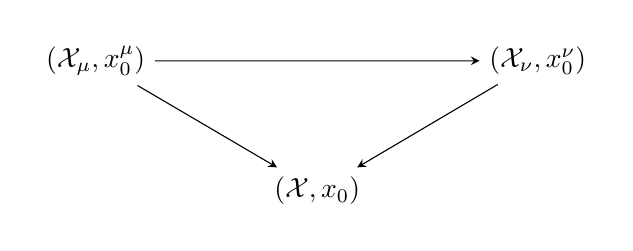
\begin{tikzpicture}
	\matrix (m) [matrix of math nodes,row sep=3em,column sep=4em,minimum width=2em]
	{
	\left(\sX_\mu, x^\mu_0 \right)   &  & \left(\sX_\nu, x^\nu_0 \right)\\ 
		& \left(\sX, x_0 \right)  &\\};
	\path[-stealth]
	(m-1-1) edge node [above] {} (m-1-3)
	(m-1-1) edge node [above]  {} (m-2-2)
	(m-1-3) edge node [right]  {} (m-2-2);
\end{tikzpicture}
\\
and then we define $\widehat \pi_1\left( \sX, x_0\right)\bydef \varprojlim G\left(\left. \sX_\la  \right| \sX\right)$. The group $\widehat \pi_1\left( \sX, x_0\right)$ is the \alert{profinite completion} $\pi_1\left( \sX, x_0\right)$. The noncommutative geometry yields finer result, i.e. one has
$
\widehat \pi_1\left( \sX, x_0\right) \bydef  \pi_1\left( \sX, x_0\right)/ \bigcap_\la \ker \left( \pi_1\left( \sX, x_0\right)\to G\left(\left. \sX_\la  \right| \sX\right)\right) 
$
To obtain an analog of algebraic geometry one needs analogs  of both: 
\begin{itemize}
	\item finite-fold coverings,
	\item diagram of pointed coverings.
\end{itemize}
\section{Finite-fold coverings}
 \begin{frame}
 	
 	\alert{Alexander Pavlov, Evgenij Troitsky}
 \begin{theorem}
 	Suppose $\mathcal X$ and $\mathcal Y$ are compact Hausdorff connected spaces and $p :\mathcal  Y \to \mathcal X$
 	is a continuous surjection. If $C(\mathcal Y )$ is a projective finitely generated Hilbert module over
 	$C(\mathcal X)$ with respect to the action
 	\begin{equation*}
 		(f\xi)(y) = f(y)\xi(p(y)), ~ f \in  C(\mathcal Y ), ~ \xi \in  C(\mathcal X),
 	\end{equation*}
 	then $p$ is a finite-fold  covering.
 \end{theorem}
  It is naturally define a finite-fold covering of $C^*$-algebras as an injective $*$-homomorphisms $A\hookto B$ such that $B$-is a finitely generated Hilbert module over
  $A$. However this definition does not gives good generalizations of results  related to topological coverings.
 
 \end{frame}
\begin{frame}
	   \begin{definition}\label{pre_defn} \alert{Pet Ivankov}.
	Let $\pi: A \hookto \widetilde{A}$ be an injective *-homomorphism of connected  $C^*$-algebras such that following conditions hold:
	\begin{enumerate}
		\item[(a)] If $\Aut\left(\widetilde{A} \right)$ is a group of *-automorphisms of $\widetilde{A}$ then the group  
		$
		G \bydef \left\{ \left.g \in \Aut\left(\widetilde{A} \right)~\right|~ ga = a;~~\forall a \in A\right\}
		$
		is finite.
		\item[(b)] 	\be\label{cond_b_eqn}
		A \cong \widetilde{A}^G\stackrel{\text{def}}{=}\left\{\left.a\in \widetilde{A}~~\right|~ a = g a;~ \forall g \in G\right\}.\ee
	\end{enumerate}
	We say that the quadruple $\left(A, \widetilde{A}, G, \pi \right)$ and/or *-homomorphism $\pi: A \to \widetilde{A}$   is a \textit{noncommutative finite-fold  pre-covering}. 
\end{definition}

\end{frame}
\begin{frame}
	\begin{definition}
		\alert{Petr Ivankov}
		Let $\left(A, \widetilde{A}, G, \pi \right)$ be a  noncommutative finite-fold  pre-covering. Suppose both $A$ and  $\widetilde{A}$ are unital. We say that $\left(A, \widetilde{A}, G, \pi \right)$ is an \textit{unital noncommutative finite-fold  covering} if \\ $\pi$ is unital and $\widetilde{A}$ is a finitely generated projective  $A$-module.
	\end{definition}
 	\begin{lemma}
		\alert{Petr Ivankov, Alexander Pavlov, Evgenij Troitsky.}
		If $\mathcal  X$ is a connected, compact, Hausdorff space then there is a natural 1-1 correspondence 
		$$
		\left(p:\widetilde{\mathcal  X}\to \mathcal  X \right)\leftrightarrow \left(C\left(\mathcal  X\right), C\left(\widetilde\sX\right), G\left(\left.\widetilde{\mathcal  X} \right|\mathcal  X\right), C_0\left(p \right)  \right).  
		$$	
		
		between finite-fold transitive coverings of $\mathcal  X$ and unital noncommutative finite-fold  coverings of $C\left(\mathcal  X\right)$.
	\end{lemma}
A covering $p:\widetilde\sX\to \mathcal  X $ is \textit{transitive}  if for all $x \in \sX$  the group $G\left(\left.\widetilde{\mathcal  X} \right|\mathcal  X\right)$ transitively acts on $p^{-1}\left( x\right)$.
\end{frame}
\begin{frame}

Above definition and lemma can be applied to compact spaces and unital $C^*$-algebras. However there is is a modification of the Definition of noncommutative finite-fold coverings with nonunital $A$ and $\widetilde{A}$.
In result one has the following Theorem.
\begin{theorem}
	\alert{P. Ivankov}. 	Let $\mathcal X$ be a connected, locally compact, Hausdorff space.
	If the  quadruple $\left(C_0\left(\mathcal  X \right), \widetilde{A}, G,    \pi\right)$ is a noncommutative finite-fold covering then there is a connected space $\widetilde{   \mathcal X }$ and a transitive finite-fold covering  $p: \widetilde{   \mathcal X } \to \sX$ such that $\widetilde{A} \cong C_0\left( \widetilde{   \mathcal X }\right)$, $G \cong G\left(\left. \widetilde{   \mathcal X } ~\right| {   \mathcal X }\right)$ and $\pi$ corresponds to $p$.
\end{theorem}
\end{frame}
\section{Pointed diagrams}

	Let us consider the following diagram\\
\begin{tikzpicture}
	\matrix (m) [matrix of math nodes,row sep=3em,column sep=4em,minimum width=2em]
	{
		\widetilde A_1  &  & \widetilde A_2\\
		& A & \\};
	\path[-stealth]
	(m-1-1) edge[dashed] node [above] {$\pi^1_2$} (m-1-3)
	(m-2-2) edge node [left]  {$\pi_1~~$} (m-1-1)
	(m-2-2) edge node [right] {$~~\pi_2$} (m-1-3);
	%\draw[dashed,->]   (m-1-1) -- (m-1-3);
\end{tikzpicture}
\\


	where $A$, $\widetilde A_1$, $\widetilde A_2$ are $C^*$-algebras and $\pi_1$, $\pi_2$, are noncommutative finite-fold coverings. We say that the unordered pair $\left( \pi_1,\pi_2\right) $ is \textit{compliant} (\alert{P. Ivankov}) if  it satisfies to following conditions:
	\begin{enumerate}
		\item[(a)]
		If there is a *-homomorphism $\pi^1_2: \widetilde A_1 \to \widetilde A_2$ such that $\pi_2 = \pi^1_2 \circ \pi_1$ then $\pi^1_2$ is  a noncommutative finite-fold  covering.
		\item[(b)] Following condition holds
		\be\label{g_sur_eqn}
		G\left(\left.\widetilde A_2~\right|A \right)\pi^1_2\left(\widetilde A_1\right)=  \pi^1_2\left(\widetilde A_1\right).
		\ee 
\pagebreak
\newline
		\item[(c)] From \eqref{g_sur_eqn} it turns out that there is the homomorphism $h: G\left(\left.\widetilde A_2~\right|A \right)\to 	G\left(\left.\widetilde A_1~\right|A \right)$ such that 
		$$
		\pi^1_2\left( h\left(g \right)a_1\right) = g \circ \pi^1_2\left(a_1 \right)
		$$
		for each $a_1 \in \widetilde A_1$.  
		We claim that $h$ is surjective. 
		\item[(d)] If  $\rho: \widetilde A_1 \to \widetilde A_2$ is any *-homomorphism  such that $\pi_2 = \rho \circ \pi_1$ then there is the unique $g \in 	G\left(\left.\widetilde A_1~\right|A \right)$ such that 
		\be\label{compliant_covering_g_eqn}
		\rho =  \pi^1_2 \circ g.
		\ee
		\newline
	\end{enumerate}
\begin{frame}
Let $A$ be a $C^*$-algebra. Below we consider a set of assumptions about $A$. If $A$ does not satisfy to this assumptions then a fundamental group of $A$ is not defined. Consider a set noncommutative finite-fold coverings $\left\{ \pi_{\la}:A \hookto A_{\la}\right\}_{\la \in \La}$ indexed by a set  $\La$ and suppose that  following conditions hold:
\begin{enumerate}
	\item[(a)] For any $\mu, \nu \in \La$ a pair $\left( \pi_\mu, \pi_\nu\right)$ is compliant.
	\item [(b)]
The set	$\La$ is a directed set ordered by the following formula.
	\be\label{fg_ord_eqn}
	\begin{split}
		\mu \ge \nu  \text{ if and only if there is an injective}\\ *-\text{homomorphism } \pi: A_\nu \hookto A_\mu; 
		\text{ such that } \pi_\mu = \pi \circ \pi_\nu.
	\end{split}
	\ee
\end{enumerate}
Consider a category $\mathfrak{S}$ such that
\begin{itemize}
	\item $\mathfrak{S}$-objects are elements of $\left\{ \pi_{\la}:A \hookto A_{\la}\right\}_{\la \in \La}$
	\item $\mathfrak{S}$-morphism from $ \pi_\nu: A \hookto A_{\nu}$ to $ \pi_\mu A \hookto A_\mu$ is an injective *-homomorphism $\pi^\nu_\mu : A_\mu \hookto  A_\nu$ such that $\pi_\nu = \pi^{\nu}_\mu \circ \pi_\nu$. 
\end{itemize}
Suppose that there is a subcategory $\mathfrak{S}^{\text{pt}}$ which is equivalent to the ordered category $\La$.

\end{frame}
\begin{frame}
	It is proven that if a category $\mathfrak{S}^{\text{pt}}$ exists then it is unique up to isomorphism. The category $\mathfrak{S}^{\text{pt}}$ is an analog of the category pointed finite-fold coverings. Moreover  one can define surjective homomorphisms  $h^\mu_\nu:  G\left(\left.A_\mu~\right|A \right) \to  G\left(\left.A_\nu~\right|A \right)$ the surjective homomorphism which come from $\pi^\nu_\mu$, hence there is the inverse limit 
	$$
	\widehat{G}=	\varprojlim_{\la \in \La} G\left(\left.A_\la~\right|~A\right)
	$$
	of groups. For any $\la \in \La$ there is the surjecive homomorphism 
	\be\label{h_la_eqn}
	h_\la:\widehat{G}\to G\left(\left.A_\la~\right|~A\right)
	\ee
	\begin{rem}
	The group $\widehat{G}$ is an analog of the obtained in the Algebraic geometry fundamental group. However we would like to obtain more accurate result.
	\end{rem}
\end{frame}
\begin{frame}
	\begin{definition}
		We say that $\mathfrak{S}$ is a \textit{category of finite-fold coverings} of $A$, $\mathfrak{S}^{\text{pt}}$ is a \textit{pointed category of finite-fold coverings} of $A$.
	\end{definition}
	
There is the natural action $\widehat{G}\times \bigcup_{\la\in \La} A_\la \to  \bigcup_{\la\in \La} A_\la$. On the other hand there is $C^*$-inductive limit $\widehat A \bydef C^*$-$\varinjlim A_\la$, such that the union $\bigcup_{\la\in \La} A_\la$ is dense in $\widehat A$. So there is a natural action $\widehat{G} \times \widehat{A}\to \widehat{A}$,.
\end{frame}
\begin{frame}
	Consider the above situation.  We say that a $C^*$-algebra $\overline A$ is \textit{ subordinated to}  $\mathfrak{S}^{\text{pt}}$ if following conditions hold:
	\begin{enumerate}
		\item [(a)] there is an inclusion $\phi: \widehat A \hookto M\left(\overline A\right)$,
		\item[(b)] there is an action $\widehat{G}\times \overline A \to \overline A$ such that
		for all $g \in \widehat{G}$,  $\quad \widehat a \in \widehat{A}$ and $\overline a \in \overline{A}$ one has
		\be\label{subord_ga_eqn}
		\begin{split}
			g\left(\phi\left(\widehat a \right)\overline{a}\right)  = 	\left(\phi\left(g\widehat a \right)\right) g \overline{a},\\
			g\left( \overline{a}\phi\left(\widehat a \right)\right) =g \overline{a}\phi\left(g\widehat a \right),
		\end{split}
		\ee
		\item[(c)] if $K\left( \overline{A}\right)$ is the Pedersen's ideal of $A$ then   for any $\la\in \La$  and $\overline a \in K\left( \overline{A}\right)$ the series $\sum_{g \in \ker\left(\widehat{G}\to G_\la\right)}g \overline a$ is convergent with respect to the strict topology of $M\left(\overline{A} \right)$. Moreover we require that
		\be\label{a_la_eqn}
		a_\la \bydef 	\bt~\text{-}\sum_{g \in \ker\left(\widehat{G}\to G_\la\right)}g \overline a \in \phi\circ \varphi_\la\left( K\left( A_\la\right) \right) 	
		\ee
		where $\varphi_\la : A_\la \hookto \widehat A$ is the natural inclusion, and $\bt$-$\sum$ means a convergence with respect to strict topology of $M\left( \overline A\right)$,
		\item[(d)] the set of given by \eqref{a_la_eqn} elements is dense in $A_\la$.
	\end{enumerate}

\end{frame}
\begin{frame}
 \begin{definition}\label{disconnected_infinite_noncommutative_covering_defn}
 	A triple
 	\be\label{disc_triple_eqn}
 \left(A, \overline{A}, G\left(\left.\overline{A}~\right| A\right)\bydef  \varprojlim_{\la\in\La}G\left(\left.A_\la~\right| A\right)\right)
 \ee
	is a \textit{disconnected universal covering} of $A$ if following conditions hold:
\begin{itemize}
	\item $\overline{A}'$ subordinated to	$A$,
	\item  for any $C^*$-algebra $\overline{A}'$ subordinated to	$A$  there is the natural injective *-homomorphism
	$\psi : \overline{A}'\hookto\overline{A}$ such that all
	$g \in \widehat{G}$,  $\widehat a \in \widehat{A}$ and $\overline a' \in \overline{A}'$ one has
	\be\label{disconnected_lim_eqn}
	\begin{split}
		g \psi\left( \overline{a}'\right) = \psi\left(g \overline{a}'\right),\\
		\psi\left(\phi'\left( \widehat  a\right)\overline a'  \right) = 	\phi\left( \widehat  a\right)\psi\left( \overline a'  \right),\\
		\psi\left(\overline a' \phi'\left( \widehat  a\right) \right) = 	\psi\left( \overline a'  \right)\phi\left( \widehat  a\right),
	\end{split}
	\ee
\end{itemize}	

\end{definition}
\end{frame}
\begin{frame}
\begin{definition}\label{connected_c_a_defn}
	We say that a $C^*$-algebra $A$ is \textit{connected} if it cannot be represented as a direct sum of $A \cong A' \oplus A''$ of nontrivial $C^*$-algebras $A'$ and $A''$.
	
	% (the Gelfand spectrum of the center of $M\left( A\right) $ is connected). Let $A \subset B$ be a connected subalgebra. We say that $A$ is a \textit{connected component} of $B$ if  $1_{M\left( A\right) }$ lies in the center of $1_{M\left( B\right) }$.
\end{definition}
\begin{definition}\label{connected_comp_defn}
	A connected closed two-sided ideal $A$ of  $C^*$-algebra $B$ is said to be a \textit{connected component of}  $B$ is there is a direct sum $B = A \oplus A'$ of $C^*$-algebras.
\end{definition}
Let $\left(A, \overline{A}, G\left(\left.\overline{A}~\right| A\right)\right)$ be a  disconnected universal covering of $A$. If $\widetilde A$ is a connected component (cf. Definition \ref{connected_comp_defn}) of $\overline{A}$, i.e. $\overline{A} = \widetilde A \oplus \widetilde A^\perp$, and
\be\label{infinite_covering_transformation_group_eqn}
G\left(\left.\widetilde{A}~\right| A\right)\bydef 
\left\{\left. g \in  G\left(\left.\overline{A}~\right| A\right)\right| \forall \widetilde a^\perp \in \widetilde A^\perp \quad g \widetilde a^\perp= \widetilde a^\perp\right\}
\ee
then there is a natural action
\be\label{gta_act_eqn}
G\left(\left.\widetilde{A}~\right| A\right)\times \widetilde{A} \to \widetilde{A}.
\ee
\end{frame}
\begin{frame}
\begin{lemma}\label{uni_dicsonnected_lem}
	If a disconnected universal covering of $A$ exists then it is unique up to *-isomorphism. 
\end{lemma}

\begin{definition}\label{good_defn}
	Let	$\mathfrak{S}^{\mathrm{pt}}$ be a pointed algebraical  finite covering category.   Suppose that $\left(A, \overline{A}, G\left(\left.\overline{A}~\right| A\right)\right)$ is a disconnected universal covering of $A$. For any $\la \in \La$ denote by $h_\la: G\left(\left.\overline{A}~\right| A\right) \to G\left(\left. A_\la~\right|~A \right)$ the natural surjective homomorphism of groups.
	We say  that $A$  is \textit{good} if  following conditions hold:
	\begin{enumerate}
		\item[(a)] if both $\widetilde{A}'$ and $\widetilde{A}''$ are  {connected components} of $\overline A$ then there is  $g \in G\left(\left.\overline{A}~\right|~ A\right)$ such that $g \widetilde{A}'= \widetilde{A}''$,
		\item [(b)] for any connected component $\widetilde A$ of $\overline{A}$ if  $G\left(\left.\widetilde{A}~\right| A\right)$ is given by  \eqref{infinite_covering_transformation_group_eqn} then for any $\la \in \La$ the restriction $h_\la|_{G\left(\left.\widetilde{A}~\right| A\right)}$ is an epimorphism, i. e. $h_\la\left(G\left(\left.\widetilde{A}~\right| A\right) \right) = G\left(\left. A_\la~\right|~A \right)$.
	\end{enumerate}
\end{definition}

\end{frame}
\begin{frame}
	\begin{definition}
	If 	$A$is a good then $G\left(\left.\widetilde{A}~\right| A\right)$ is said to be the \textit{fundamental group} of $A$. We write
	$$
\pi_1\left(A \right) \bydef G\left(\left.\widetilde{A}~\right| A\right).	
	$$
	\end{definition}
\end{frame}
\section{Commutative case}
\begin{frame}
	\begin{definition}\label{top_weakly_semi1_defn}
		An open connected subset $\sU\subset \sX$ of a topological space is said to be \textit{semilocally proper} if it is evenly covered by any transitive covering $\widetilde{\sX}\to\sX$.	A space $\sX$ is said to be \textit{weakly semilocally 1-connected} if for  every point $x\in \sX$ there is a semilocally proper neighborhood.
	\end{definition} 
	Let $\sX$ be a connected, locally connected, locally compact, Hausdorff  topological space. Consider a category $\mathfrak{S}_\sX$, such that 
	\begin{itemize}
		\item  $\mathfrak{S}_\sX$-objects are transitive  finite-fold coverings $p:\widetilde \sX \to \sX$,
		\item  $\mathfrak{S}_\sX$-morphism from  $p':\widetilde \sX' \to \sX$ to  $p'':\widetilde \sX \to \sX$ is a surjective continuous map $p: \widetilde \sX' \to \widetilde \sX''$, such that $p' = p \circ p''$.
	\end{itemize}
It is proven that $p$ is transitive covering.	There is a pre-ordering  on a family of  $\mathfrak{S}_\sX$-objects such that $\left( \widetilde \sX' \to \sX\right) \ge \left( \widetilde \sX' \to \sX\right)$ if and only is there is a  $\mathfrak{S}_\sX$-morphism from  $p':\widetilde \sX' \to \sX$ to  $p'':\widetilde \sX'' \to \sX$. This pre-ordering corresponds to a directed set $\La$.
\end{frame}
\begin{frame}
Suppose that the set of  $\mathfrak{S}_\sX$-objects is indexed by $\La$, i.e. 
$$
\mathfrak{S}_\sX\text{-objects} = \left\{\sX_\la \to\sX \right\}_{\la \in \La}.
$$
Assume that for any $\la\in \La$ there is a base point $x^\la_0\in \sX_\la$ and one has a subcategory 
of pointed maps $\mathfrak{S}_{\left(\sX, x_0\right)}$ such that:
\begin{itemize}
	\item  a set  $\mathfrak{S}_{\left(\sX, x_0\right)}$-objects coincides with a set of  $\mathfrak{S}$-objects.
	\item any $\mathfrak{S}_{\left(\sX, x_0\right)}$-morphism is a pointed map $\left(\sX_\nu, x^\nu_0\right)\to \left(\sX_\mu, x^\mu_0\right)$.
\end{itemize}
The category $\mathfrak{S}_{\left(\sX, x_0\right)}$ is equivalent to the pre-ordering category $\La$.
A category $\mathfrak{S}_\sX$ yields a category $\mathfrak{S}$ of {category of finite-fold coverings} of $C_0\left(\sX \right)$ such that 
\begin{itemize}
	\item $\mathfrak{S}$ - objects are noncommutative finite-fold coverings $\left(C_0\left( \sX\right), C_0\left( \sX_\la\right),  G\left(\left. \sX_\la  \right| \sX\right), \pi_\la   \right)$.
	\item $\mathfrak{S}$-morphism is from $\left(C_0\left( \sX\right), C_0\left( \sX_\nu\right),  G\left(\left. \sX_\nu  \right| \sX\right), \pi_\nu   \right)$ to $\left(C_0\left( \sX\right), C_0\left( \sX_\mu\right),  G\left(\left. \sX_\mu  \right| \sX\right), \pi_\mu   \right)$ is an induced by a covering $\sX_\nu \to \sX_\mu$ injective $*$-homomorphism $ C_0\left( \sX_\mu\right) \hookto  C_0\left( \sX_\nu\right)$.
\end{itemize}
A subcategory $\mathfrak{S}_{\left(\sX, x_0\right)}$ of $\mathfrak{S}_\sX$ induces  a {pointed  finite-fold coverings} $\mathfrak{S}^{\mathrm{pt}}$ of coverings of $C_0\left(\sX \right)$.
\end{frame}
\begin{frame}
Now we have all ingredients to obtain fundamental group of $C^*$-algebra as profinite completion. However we can have more accurate result.

\begin{definition}\label{top_specp_defn}
Let $\widehat \sX\bydef \varprojlim_{\la \in \La}\sX_\la$ be the inverse limit of topological spaces. Let $\widehat p_\la : \widehat \sX\to \sX_\la$ be the natural continuous map for all $\la\in\La$. The subset  $\widehat \sU\subset \widehat \sX$ 
	is said to be \textit{special} if for all $\la\in\La$ on has:
	\begin{itemize}
		\item $\widehat p_\la \left(\widehat\sU\right)$ is an open,  connected subspace of $\sX_\la$ and the a set 
		$p_\la\circ \widehat p_\la\left(\widehat \sU \right)$ is   semilocally {proper}, 		\item  the natural map $\widehat \sU \to  \widehat p_\la\left(\widehat \sU \right)$ is bijective.
	\end{itemize}
\end{definition}
\end{frame}
\begin{frame}
\begin{lemma}
The set of special sets is a base of topology on the set $\widehat \sX$.
\end{lemma}
\begin{definition}
Consider a topological space  $\overline  \sX$ which coincides with $\widehat \sX$ as a set and the topology $\overline \sX$ is generated by special sets. We say that $\overline  \sX$ is a \textit{disconnected universal covering of} $\sX$. Any connected component $\widetilde \sX$ of $\overline  \sX$ is is a \textit{connected universal covering of} $\sX$
\end{definition}
\begin{lemma}
	For any $\la\in \La$ both  natural maps $\overline p_\la: \overline  \sX \to \sX_\la$  and $\widetilde p_\la: \widetilde  \sX \to \sX_\la$ are transitive coverings. Moreover one has
\be\nonumber
\begin{split}G\left(\left. \overline\sX  \right| \sX\right)= \varprojlim_{\la \in \La} G\left(\left. \sX_\la  \right| \sX\right)\\G\left(\left. \widetilde\sX  \right| \sX\right) =  \frac{\pi_1\left( \sX, x_0\right)}{ \bigcap_{\la\in \La} \ker \left( \pi_1\left( \sX, x_0\right)\to G\left(\left. \sX_\la  \right| \sX\right)\right)}. 
\end{split}
\ee
\end{lemma}


\end{frame}
\begin{frame}
Since for all $\la\in \La$ a map $\overline p_\la: \overline  \sX \to \sX_\la$ 
continuous is an injective $*$-homomorphism  $C_0\left(\sX_\la \right)\hookto C_b \left( \overline  \sX\right) = M\left(C_0 \left( \overline  \sX\right) \right)$. From this fact one can deduce  that there is an  injective $*$-homomorphism  $\phi: C^*$-$\varinjlim_{\la\in \La} C_0\left(\sX_\la \right)\hookto M\left(C_0 \left( \overline  \sX\right) \right)$. From $G\left(\left. \overline\sX  \right| \sX\right)= \varprojlim_{\la \in \La} G\left(\left. \sX_\la  \right| \sX\right)$ it follows that there is  an action
$$
\widehat G \times C_0 \left( \overline  \sX\right) \to C_0 \left( \overline  \sX\right).
$$
where $\widehat G \bydef \varprojlim_{\la \in \La} G\left(\left. \sX_\la  \right| \sX\right)$.
Moreover
for all $g \in \widehat{G}$,  $\quad \widehat a \in \widehat{A}$ and $\overline a \in \overline{A}$ one has
\be\nonumber
\begin{split}
	g\left(\phi\left(\widehat a \right)\overline{a}\right)  = 	\left(\phi\left(g\widehat a \right)\right) g \overline{a},\\
	g\left( \overline{a}\phi\left(\widehat a \right)\right) =g \overline{a}\phi\left(g\widehat a \right).
\end{split}
\ee
(cf. equation \eqref{disconnected_lim_eqn}).
\end{frame}
\begin{frame}
\begin{lemma}
	If $\overline  \sY \subset \overline  \sX$ is a compact set then there is $\la \in \La$ such that
	for any $\mu \ge \la$ the set $\overline  \sY$ is mapped homeomorphically onto $\overline p_\mu \left( \overline  \sY\right)\subset \sX_\mu$. 
\end{lemma}
\end{frame}

\begin{corollary}
For any $\overline a \in C_c\left( \overline  \sX\right) = K\left(C_0\left( \overline  \sX\right)  \right)$ and any $\la \in \La$ the series
$$
\sum_{g \in \ker\left( \widehat G \to G\left(\left. \sX_\la  \right| \sX\right)\right) } g \overline a
$$
is convergent with respect to the strict topology of $M\left(C_0\left( \overline  \sX\right) \right)$. Moreover there is $a_\la\in C_c\left(\sX_\la \right)$ such that $\phi\left(a_\la \right)$ is the sum of the series.  
\end{corollary}

From  $\overline a \in C_c\left( \overline  \sX\right)$ it follows that the support $\overline \sY$ of $\overline a$ is compact. Let us prove this statement for special cases of $\la \in \La$  such that  $\overline  \sY$ is mapped homeomorphically onto $\overline p_\la \left( \overline  \sY\right)\subset \sX_\la$. If $a_\la \in C_c\left(\sX_\la \right)$ is such that
$$
a_\la\left(x_\la \right) = \begin{cases}
	\overline a\left( \overline x\right)  &  \overline x \in  \overline \sY \quad \text { AND } \quad \overline p_\la\left( \overline x \right)= x_\la \\
	0 & x_\la \notin  p_\la \left( \overline  \sY\right)
\end{cases}
$$

then one can proof that the strict limit of the series equals to $\phi\left(a_\la \right)$. Another cases can be deduced from special ones.
\begin{frame}
From the above constructions it follows that the $C^*$-algebra $C_0\left( \overline \sX\right)$ is subordinated to   $\mathfrak{S}^{\text{pt}}$. It is much more difficult to prove that $C_0\left( \overline \sX\right)$ is the unique up to isomorphism $C^*$-algebra subordinated to   $\mathfrak{S}^{\text{pt}}$. It follows that the triple
	\be\nonumber
\left(C_0\left(  \sX\right), C_0\left( \overline \sX\right), G\left(\left.\overline{\sX}~\right| \sX\right)\right)
\ee
is a {disconnected universal covering} of $A$ (cf. equation \ref{disc_triple_eqn}). If $\widetilde \sX$ is a connected component of $\overline \sX$ then there is a covering  $\widetilde \sX\to \sX$ because $ \sX$ is locally connected. If both $\widetilde \sX'$ and $\widetilde \sX''$ are connected components of $\overline \sX$,  both $\widetilde x'_0 \in \widetilde \sX'$ and $\widetilde x''_0 \in \widetilde \sX''$ are such that $\overline p\left( \widetilde x'_0\right)= \overline p\left( \widetilde x''_0\right)$ then there is  $g \in G\left(\left.\overline{\sX}~\right| \sX\right)$ such that $ \widetilde x''_0 = g  \widetilde x'_0$. From this fact one can obtain a following
\be
\begin{split}
\widetilde \sX'' = g \widetilde \sX',\quad 
C_0\left( \widetilde \sX''\right) = gC_0\left( \widetilde \sX'\right).
\end{split}
\ee
Since connected components of $C_0\left( \overline \sX\right)$ correspond to connected components of $\overline \sX$ and taking into account that the homomorphisms $G\left(\left.\widetilde{\sX}~\right| \sX\right)\to G\left(\left.{\sX}_\la~\right| \sX\right)$ is surjective the $C^*$-algebra $C_0\left( \sX\right)$ is good. 
\end{frame}
\begin{frame}
\be\nonumber
G\left(\left.\widetilde{A}~\right| A\right)\bydef 
\left\{\left. g \in  G\left(\left.\overline{A}~\right| A\right)\right| \forall \widetilde a^\perp \in \widetilde A^\perp \quad g \widetilde a^\perp= \widetilde a^\perp\right\}
\ee

(cf. equation \ref{infinite_covering_transformation_group_eqn})
\end{frame}



\end{document}























